%----------------------------------------------------------------------------------------
% Research Proposal for MUST 
%
% Title:
%
% Author:HE PEILIN
%
% Last modified: 2022-04-05
%-----------------------------------------------------------------------------------------
\documentclass[12pt, a4paper]{report}
\pagestyle{headings}

\pagestyle{headings}

% Note that the line below could be modified to suit a
% particular system since the "geometry" package behaves
% differently in Unix, Windows and Mac, especially for the
% top margins.
% Adjust the parameter "top" (measuring the height of the
% space allocated to a header) and "headsep" (measuring
% the distance from the bottom of the header to the
% first line of text.
%\usepackage[top=2.5cm,left=3.8cm,bottom=2.5cm,right=2.5cm,headsep=0.2in]{geometry}

\usepackage{setspace}
%\renewcommand{\baselinestretch}{1.5}


\doublespacing

% Headers and footers for thesis
\usepackage{fancyhdr}

\markboth{}{}
\newcommand\startchapter[1]{\chapter{#1}\thispagestyle{myheadings}}
\newcommand\startappendix[1]{\chapter{#1}\thispagestyle{myheadings}}
\newcommand\startfirstchapter[1]{\chapter{#1}}

% Manual addition of section to Table of Contents
\newcommand\TOCadd[1]{\newpage\phantomsection\addcontentsline{toc}{chapter}{#1}}

% Float Customization
\renewcommand{\floatpagefraction}{0.01}

% Customization of Tables of Contents and List of Figures/Tables
\usepackage[labelsep=space]{caption}

%\usepackage{tocloft}
\usepackage[titles,subfigure]{tocloft}

\renewcommand{\cftchappresnum}{Chapter\ }
\renewcommand\cftchapnumwidth{1.15in}
\makeatletter
\newcommand*\updatechaptername{%
   \addtocontents{toc}{\protect\renewcommand*\protect\cftchappresnum{\@chapapp\ }}
   } \makeatother
\renewcommand\cfttabpresnum{Table\ }
\renewcommand\cfttabnumwidth{0.75in}
\renewcommand\cftfigpresnum{Figure\ }
\renewcommand\cftfignumwidth{1in}

%%% configure font size
\newcommand{\sizefont}[1]{\fontsize{#1}{\baselineskip}\selectfont}%

\newcommand{\mycell}[3]{
	\makecell*[l{p{2.25cm}}]{#1\\[2mm] #2}
	&\hspace{-2mm} \textbf{:}    
	&\hspace{-8mm}\makecell*[c{p{22em}}]{\centering{\vspace{.5mm} #3}\\ \rule[-.25mm]{7cm}{.4mm}} \\[2mm]
}



\usepackage{appendix}

%bib format
\usepackage[sort&compress,comma,square,numbers]{natbib}
\usepackage{apalike}

% Long Table and decimal aligned columns
\usepackage{dcolumn}
\usepackage{longtable}
\usepackage{multirow}
\usepackage{morefloats}
\usepackage{makecell}
\usepackage{minibox}
\usepackage{tabularx} %\table 
\usepackage{booktabs}% 	\toprule \midrule \bottomrule
\usepackage{xltabular}
\usepackage{array}
\usepackage{enumitem}

% define color canvas 
\usepackage[table]{xcolor}
\usepackage{colortbl}
\definecolor{mygray}{gray}{.9}
\definecolor{mypink}{rgb}{.99,.91,.95}
\definecolor{mycyan}{cmyk}{.3,0,0,0}


% Mathematics support
\usepackage{amsmath}
\usepackage{amsthm}
\usepackage{amssymb}
\usepackage{amsfonts}
\usepackage{amscd}
\usepackage{verbatim}

% algorithms algorithm2e &algopseudocode
\makeatletter  
\newif\if@restonecol  
\makeatother  
\let\algorithm\relax  
\let\endalgorithm\relax 
\usepackage[boxed,ruled,noline,linesnumbered,commentsnumbered]{algorithm2e}
\usepackage{algpseudocode}

% tikz 
\usepackage{tikz}
\usetikzlibrary{bending,intersections,calc,graphs,arrows,arrows.meta,decorations.pathmorphing,backgrounds,positioning,fit,petri,matrix,shapes}


% Text Control
\usepackage{xspace}
\usepackage{textcase}
\usepackage[english]{babel}
% \usepackage[T1]{fontenc}
% \usepackage{txfonts}

% Theorem initialization 
\newtheorem{theorem}{Theorem}
\newtheorem{corollary}[theorem]{Corollary}
\newtheorem{lemma}[theorem]{Lemma}
\newtheorem{definition}{Definition}

% Graphics
\usepackage{wasysym}
\usepackage{graphics}
\usepackage{graphicx}   % A package to allow insertion of external image files
\DeclareGraphicsExtensions{.pdf, .jpg, .tif, .png, .gif}  
\usepackage{wrapfig}
\usepackage{rotating}
% \usepackage{subfigure}
\usepackage{subfig}
\usepackage{epsfig}

% text colour
\usepackage{color}
\usepackage[colorlinks,linkcolor=black,anchorcolor=red,filecolor=magenta,urlcolor=cyan,citecolor=blue]{hyperref}   
%\PassOptionsToPackage{usenames, dvipsnames}{xcolor} %\usepackage[usenames,dvipsnames]{xcolor}

% bookmarks
\usepackage{setspace}

% code listing 
\usepackage{listings}
\lstset{
	tabsize=2,
	numbers=left, 
	numberstyle= \tiny, 
	rulesepcolor=\color{red!20!green!20!blue!20},
	keywordstyle=\color{blue!90}\bfseries , 
	commentstyle=\color{red!10!green!70}\textit , 
	showspaces=false,    
	showstringspaces=false,  
	frame=shadowbox,
	breaklines=true,
	extendedchars=false, 
	% title=\lstname ,
	% morekeywords={*,...}               % if you want to add more keywords to the set
}

% pdf & title
\usepackage{epstopdf}
\usepackage{tabu}
\usepackage{wallpaper}
\usepackage[center]{titlesec}
\usepackage{fancyhdr}
\usepackage{pdfpages}
\usepackage{titlesec}


% traditional chinese font 
\usepackage{textcomp}
\usepackage{xeCJK,CJKnumb,CJK}
\usepackage{fontspec}


\usepackage{Proposal}
\usepackage{titlepage}
\usepackage{cv-structure}


% \setCJKmainfont[AutoFakeSlant=0.3, AutoFakeBold=2.17,Path=fonts/]{KaiTi}
\setmainfont{Times New Roman}

\lhead{\tiny }
\chead{}
\rhead{\small \leftmark}
\renewcommand{\headrulewidth}{1pt}

%\CenterWallPaper{.6}{figure/waterlogo.jpg}
\graphicspath{{.}}

\renewcommand{\baselinestretch}{1.5}
\parindent=0pt


%\makeatletter %使\section居中
%\renewcommand{\section}{\@startsection{section}{1}{0mm}
 % {-\baselineskip}{0.5\baselineskip}{\bf\leftline}}
% {-\baselineskip}{0.5\baselineskip}{\bf\centerline}}
%\makeatother
%使\chapte左侧
%\titleformat{command}[shape]{format}{label}{sep}{before}[after]

%\titlecontents{chapter}% <section-type>
%  [0pt]% <left>
%  {}% <above-code>
%  {\bfseries\chaptername\ \thecontentslabel\quad}% <numbered-entry-format>
%  {\bfseries}% <numberless-entry-format>
%  {\bfseries\hfill\contentspage}% <filler-page-format>

\titleformat{\chapter}{\centering\Large\bfseries}{Chapter\,\thechapter.}{1em}{}
%\titleformat{\chapter}{\centering\Large\bfseries}{\thechapter.}{1em}{}
\titlespacing{\chapter}{0pt}{0em}{1em}[0pt]

%\titleformat{\section}{\leftline\bfseries}{section\,\thesection}{1em}{}

\makeatletter %使\section左侧
\renewcommand{\section}{\@startsection{section}{1}{0mm}
 {-\baselineskip}{0.5\baselineskip}{\Large\bf\leftline}}
 %{-\baselineskip}{0.5\baselineskip}{\Large\bf\centerline}}
\makeatother


\makeatletter %使\subsection左侧
\renewcommand{\subsection}{\@startsection{subsection}{1}{0mm}
  {-\baselineskip}{0.5\baselineskip}{\large\bf\leftline}}
 %{-\baselineskip}{0.5\baselineskip}{\bf\centerline}}
\makeatother

\makeatletter %\subsubection居中,Roman
\renewcommand{\subsubsection}{\@startsection{subsubsection}{1}{0mm}
 {-\baselineskip}{0.5\baselineskip}{\bf\centerline}}
\renewcommand{\thesubsubsection}{\Roman{subsubsection}} 
\makeatletter


\begin{document}
%\bibliographystyle{alpha}
\thispagestyle{empty}

% --------------------------
% def information 

\def\Ctitle         {中文題目}
\def\Etitle         {GANxxxxx}
\def\Cname 			{某某某}
\def\Ename          {HE}
\def\Stuno 			{18098xxx-xxxx-xxxx}
\def\Faculty 		{xxxx}
\def\Program 		{xxx}
\def\Major 		{xxxx}
\def\SupervisorC	{xxxx}
\def\SupervisorE	{xxxx}
\newcommand{\Stoday}{\number\year 年 \number\month 月 \number\day 日}

%% Traditional Chinese title
%%%%%%%%%%%%%%%%%%%%%%%%%%%%%%%%%%%%%%%%%%%%%%%%%%%%%%%%%%%%%%%%%%
\begin{titlepage}
\CenterWallPaper{.6}{figure/waterlogo.jpg}
\thispagestyle{empty} 														
\titleofthesisC								
\end{titlepage}

%-------------------------------------------------------------------------------------
\begin{titlepage}
\CenterWallPaper{.6}{figure/waterlogo.jpg}
\thispagestyle{empty} 
\titleofthesisE
\end{titlepage}

%-------------------------------------------------------------------------------------

\pagestyle{fancy}
\pagenumbering{Roman}
\setlength{\parindent}{0.6cm}
\addcontentsline{toc}{chapter}{摘要}

\lhead{\Etitle}
\rhead{\small 摘要}
\setlength{\parskip}{0pt}    
\chapter*{摘要} \par
\bigskip
\hspace*{1em}

摘要

\vspace{2em}
\par \noindent\textbf{關鍵詞: XXXX}
%\end{abstract}

%-------------------------------------------------------------------------------------
\newpage
\pagestyle{fancy}
%\pagenumbering{roman}
%\setlength{\parindent}{0.6cm}
\addcontentsline{toc}{chapter}{Abstract}

\lhead{\Etitle}
\rhead{\small Abstract}
\setlength{\parskip}{0pt}

\chapter*{Abstract} \par
\bigskip
\hspace*{1em}
Abstract

\vspace{2em}
\par \noindent\textbf{Keywords: XXXX}


%-------------------------------------------------------------------------------------
\newpage
\pagestyle{fancy}
%\lhead{\tiny }
%\chead{}
%\rhead{\small \leftmark}
\addcontentsline{toc}{chapter}{Contents}

\lhead{\Etitle}
\rhead{\small Contents}
    \setlength{\parskip}{0pt}

%\thispagestyle{plain}
\tableofcontents

%\thispagestyle{plain}
%-------------------------------------------------------------------------------------


\newpage

\addcontentsline{toc}{chapter}{List of Figures}

\listoffigures

\lhead{\Etitle}
\rhead{\small List of Figures}
    \setlength{\parskip}{0pt}

%-------------------------------------------------------------------------------------
%\thispagestyle{plain}
\newpage
%\thispagestyle{plain}
\addcontentsline{toc}{chapter}{List of Tables}

\listoftables

\lhead{\Etitle}
\rhead{\small List of Tables}
    \setlength{\parskip}{0pt}


%\thispagestyle{plain}
%\newpage
%\pagestyle{headings}
%-------------------------------------------------------------------------------------
\pagestyle{fancy}
%------------------------------------------------------------------------------------------------------------------------------------------------------------------------------------------------------------------------------------
\newpage
\chapter{Chapter one}


\pagenumbering{arabic}


\lhead{\Etitle}
\rhead{\small Chapter one}
    \setlength{\parskip}{0pt}
   
Chapter one's contents. There is the citation. \cite{DBLP:journals/corr/ReedAYLSL16,7780634}

\begin{itemize}
    \item Introduction
    \item Related work
    \item Background
    \item Notation
    \item Method
    \item Experiment
    \item Conclusion
\end{itemize}

\begin{enumerate}
    \item Introduction
    \item Related work
    \item Background
    \item Notation
    \item Method
    \item Experiment
    \item Conclusion
\end{enumerate}

%-----------------------------------------------------------------------------------------------------------------------------------------------------------------------------------------------------------------------------------

%\thispagestyle{plain}

%-----------------------------------------------------------------------------------------------------------------------------------------------------------------------------------------------------------------------------------
\newpage
\chapter{Chapter two}
%\thispagestyle{plain}
\lhead{\Etitle}
\rhead{\small Chapter two}
    \setlength{\parskip}{0pt}

Chapter two'contents.

\section{Section two}\label{Section_two}

\subsection{Table}

Subsection's contents in Table \ref{tab:mul-tab} and \ref{tab:Ntt} .

\begin{table}
    %\Large
    \fontsize{7}{15}\selectfont
    \begin{center}
 %   \begin{tabular}{|c|c|c|c|c|c|c|c|c|c|c|c|c|c|c| p{0.5cm}|}
    \caption[Comparison of the APs and mAPs with our framework and those from DPM and R-CNN.]{Comparison of the APs and mAPs with our framework and those from DPM and R-CNN on PASCAL VOC 2007 testing dataset.}\label{tab:mul-tab}
    \begin{tabu} to 1.00\textwidth{|X[c]|X[c] X[c] X[c] X[c] X[c] X[c] X[c] p{0.5cm}|}
    \hline
      &plane&bike&bird&boat&bottle&bus&car&cat \\ \hline
      DPM&0.0&0.0&0.0&0.0&0.0&0.0&0.0&0.0 \\ \hline
      R-CNN&0.0&0.0&0.0&0.0&0.0&0.0&0.0&0.0 \\ \hline
      Ours&{\bf0.0}&{\bf0.0}&{\bf0.0}&{\bf0.0}&{\bf0.0}&{\bf0.0}&{\bf0.0}&{\bf0.0} \\ \hline
 %   \end{tabular}
    \end{tabu}

    \vspace{1cm}

    \begin{tabu} to 1.00\textwidth{|X[c]|X[c] X[c] X[c] X[c] X[c] X[c] X[c] p{0.5cm}|}
    \hline
      &chair&cow&table&dog&horse&mbik&pers&plant \\ \hline
      DPM&0.0&0.0&0.0&0.0&0.0&0.0&0.0&0.0 \\ \hline
      R-CNN&0.0&0.0&0.05&56.1&60.6&66.8&54.2&{\bf0.0} \\ \hline
      Ours&{\bf0.0}&{\bf0.0}&{\bf0.0}&{\bf0.0}&{\bf0.0}&{\bf0.0}&{\bf0.0}&0.0 \\ \hline
 %   \end{tabular}
    \end{tabu}

    \end{center}

\end{table}

\def\degree{${}^\circ$}
\begin{table}[h]
	\begin{center}
		\begin{tabularx}{\textwidth}{cX}
			\toprule
			\multicolumn{1}{m{3cm}}{\centering Symbol}
			&\multicolumn{1}{m{15cm}}{\centering Definition}\\
			\midrule      
			$s$&Angles of 45\degree in n-polygon \\
			$r$&Angles of 90\degree in n-polygon\\
			$l$&Angles of 135\degree in n-polygon\\
			$S$& The aggregate of all space not matched any piece   \\
			$P$& The aggregate of the weight point position in two-dimensional array\\
			$H$& Threshold evaluating the probability to search next state\\
			$\eta(p,d)$&Thresholding function of Simulated Annealing\\		
			\bottomrule
		\end{tabularx}
		\caption{Notations}\label{tab:Ntt}
	\end{center}
\end{table}

\subsection{Algorithms}

Subsection's contents.

The Algorithms \ref{algo:intervalR} and Algorithms \ref{algo:function}: 
\begin{algorithm}
    \DontPrintSemicolon
    %%%%%%%%%%%%%
    % set keywords arguments
    \KwData{$G=(X,U)$ such that $G^{tc}$ is an order.}
    \KwResult{$G'=(X,V)$ with $V\subseteq U$ such that $G'^{tc}$ is an
    interval order.}
    %%%%%%%%%%%%%%%%%%%%%%%%%%%%%%%%%%%%%%%%%%%
    \Begin{
    $V \longleftarrow U$\;
    $S \longleftarrow \emptyset$\;
    \For{$x\in X$}{
    $NbSuccInS(x) \longleftarrow 0$\;
    $NbPredInMin(x) \longleftarrow 0$\;
    $NbPredNotInMin(x) \longleftarrow |ImPred(x)|$\;
    }
    \For{$x \in X$}{
    \If{$NbPredInMin(x) = 0$ {\bf and} $NbPredNotInMin(x) = 0$}{
    $AppendToMin(x)$}
    }
    \nl\While{$S \neq \emptyset$}{\label{InRes1}
    \nlset{REM} remove $x$ from the list of $T$ of maximal index\;\label{InResR}
    \lnl{InRes2}\While{$|S \cap ImSucc(x)| \neq |S|$}{
    \For{$ y \in S-ImSucc(x)$}{
    \{ remove from $V$ all the arcs $zy$ : \}\;
    \For{$z \in ImPred(y) \cap Min$}{
    remove the arc $zy$ from $V$\;
    $NbSuccInS(z) \longleftarrow NbSuccInS(z) - 1$\;
    move $z$ in $T$ to the list preceding its present list\;
    \{i.e. If $z \in T[k]$, move $z$ from $T[k]$ to
    $T[k-1]$\}\;
    }
    $NbPredInMin(y) \longleftarrow 0$\;
    $NbPredNotInMin(y) \longleftarrow 0$\;
    $S \longleftarrow S - \{y\}$\;
    $AppendToMin(y)$\;
    }
    }
    $RemoveFromMin(x)$\;
    }
    }
    \caption{IntervalRestriction\label{IR}}
    \label{algo:intervalR}
\end{algorithm}
    
\begin{algorithm}
    %%%%%%%%%%%%%
    % set keywords function 
    \SetKwProg{Fn}{Function}{ is}{end}
    \newcommand{\forcond}{$i=0$ \KwTo $n$}
    \SetKwFunction{FRecurs}{FnRecursive}%
    %%%%%%%%%%%%%%%%%%%%%%%%%%%%%%%%%%%%%%%%%%
    \Fn(\tcc*[h]{algorithm as a recursive function}){\FRecurs{some args}}
    {
        \KwData{Some input data\\these inputs can be displayed on several lines and one
        input can be wider than line's width.}
        \KwResult{Same for output data}
        \tcc{this is a comment to tell you that we will now really start code}
        \If(\tcc*[h]{a simple if but with a comment on the same line}){this is true}
        {
            we do that, else nothing\;
            \tcc{we will include other if so you can see this is possible}
            \eIf{we agree that}
            {
                we do that\;
            }
            {
            else we will do a more complicated if using else if\;
            \uIf{this first condition is true}
            {
                we do that\;
            }
            \uElseIf{this other condition is true}
            {
                this is done\tcc*[r]{else if}
            }
            \Else
            {
                in other case, we do this\tcc*[r]{else}
            }
            }
        }
        \tcc{now loops}
        \For{\forcond}
        {
            a for loop\;
        }
        \While{$i<n$}{
        a while loop including a repeat--until loop\;
            \Repeat{this end condition}
            {
                do this things\;
            }
        }
        They are many other possibilities and customization possible that you have to
        discover by reading the documentation.
    }
    \caption{Algorithm as a Recursive Function}
    \label{algo:function}
\end{algorithm}



\subsection{Figure}
Figure contents

\subsubsection{Subfigure}
In Figure \ref{fig:MUST1} and Figure \ref{fig:MUST2}, ....

\begin{figure}[!htbp]
	\begin{minipage}[t]{0.5\linewidth}
		\centering
		
\includegraphics[width=\textwidth]{figure/MUSTSchoolBadgecolor.pdf}
	\end{minipage}
	\begin{minipage}[t]{0.5\linewidth}
		\centering
		
\includegraphics[width=\textwidth]{figure/MUSTSchoolBadgecolor.pdf}
	\end{minipage}
	\caption{MUSTSchoolBadgecolor.pdf} 
	\label{fig:MUST1}
\end{figure}

\begin{figure}[!htbp]
	\begin{minipage}[t]{0.5\linewidth}
		\centering
		
\includegraphics[width=\textwidth]{figure/MUSTSchoolBadgecolor.pdf}
	\end{minipage}
	\begin{minipage}[t]{0.5\linewidth}
		\centering
		
\includegraphics[width=\textwidth]{figure/MUSTSchoolBadgecolor.pdf}
	\end{minipage}
	\begin{minipage}[t]{0.5\linewidth}
		\centering
		
\includegraphics[width=\textwidth]{figure/MUSTSchoolBadgecolor.pdf}
	\end{minipage}
    \begin{minipage}[t]{0.5\linewidth}
		\centering
		
\includegraphics[width=\textwidth]{figure/MUSTSchoolBadgecolor.pdf}
	\end{minipage}
	\caption{MUSTSchoolBadgecolor.pdf - 2 }
	\label{fig:MUST2}
\end{figure}

\subsubsection{Tikz Figure}
In Figure \ref{fig:flowchart} \footnote{referred from \url{https://latexdraw.com/draw-flowcharts-latex-tutorial/}}  ....
\begin{figure}
    \centering
    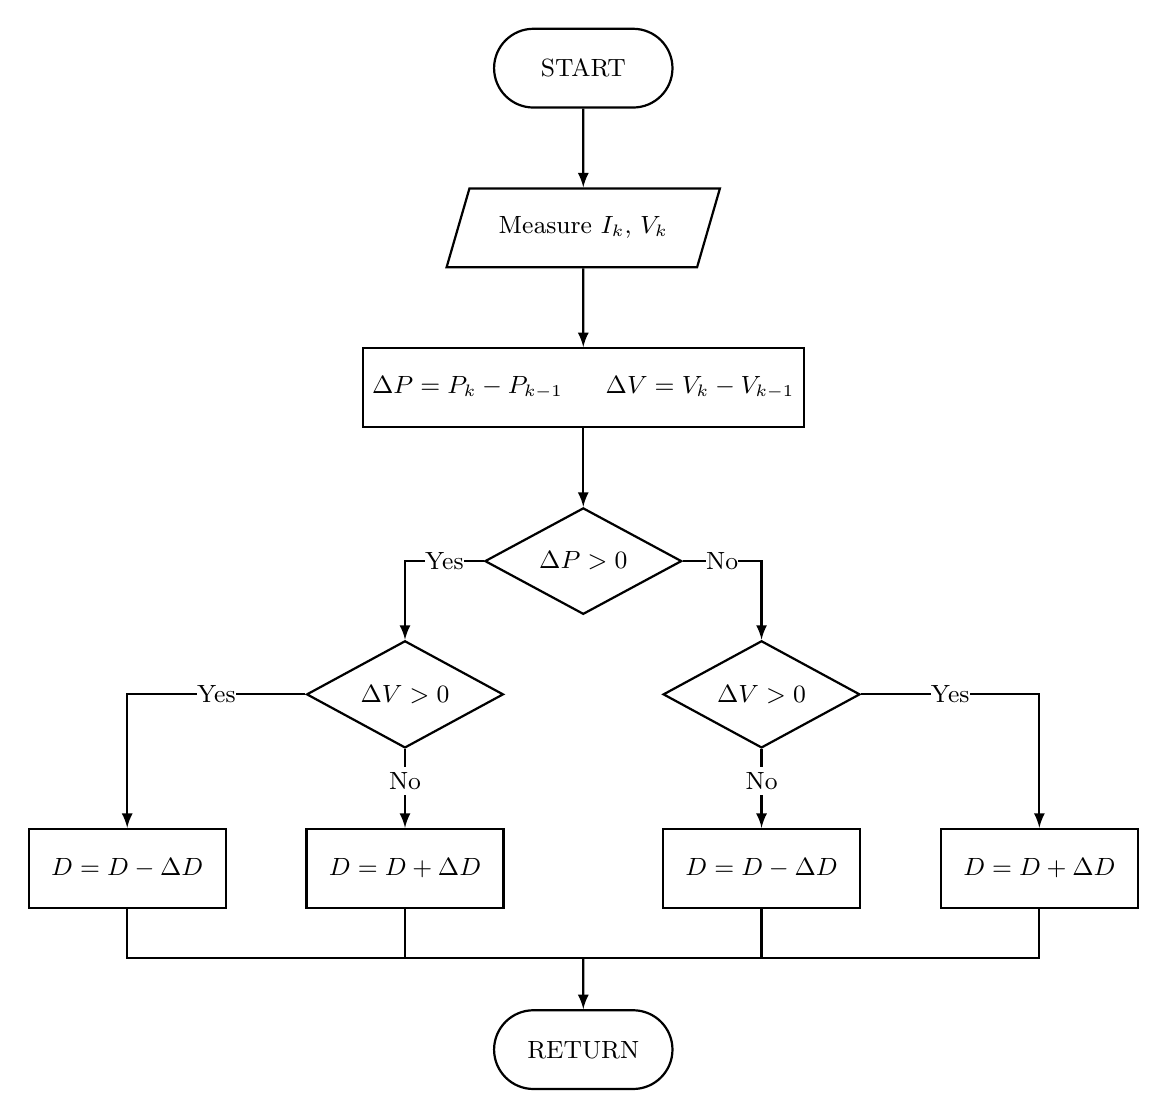
\begin{tikzpicture}[font=\small,thick]
        % Start block
        \node[draw,
        rounded rectangle,
        minimum width=2.5cm,
        minimum height=1cm] (block1) {START};
        
        % Voltage and Current Measurement
        \node[draw,
        trapezium, 
        trapezium left angle = 65,
        trapezium right angle = 115,
        trapezium stretches,
        below=of block1,
        minimum width=3.5cm,
        minimum height=1cm
        ] (block2) { Measure $I_k$, $V_k$ };

        % Power and voltage variation
        \node[draw,
        below=of block2,
        minimum width=3.5cm,
        minimum height=1cm
        ] (block3) { $\Delta P=P_k-P_{k-1}$ \hspace{1em} $\Delta V=V_k-V_{k-1}$ };

        % Conditions test
        \node[draw,
        diamond,
        below=of block3,
        minimum width=2.5cm,
        inner sep=0] (block4) { $\Delta P>0$};

        \node[draw,
        diamond,
        below left=of block4,
        minimum width=2.5cm,
        inner sep=0] (block5) { $\Delta V>0$};

        \node[draw,
        diamond,
        below right=of block4,
        minimum width=2.5cm,
        inner sep=0] (block6) { $\Delta V>0$};

        % Increase and Decrease duty cycle
        \node[draw,
        below=of block5,
        minimum width=2.5cm,
        minimum height=1cm] (block7) { $D=D+\Delta D$};

        \node[draw,
        left=of block7,
        minimum width=2.5cm,
        minimum height=1cm] (block8) { $D=D-\Delta D$};

        \node[draw,
        below=of block6,
        minimum width=2.5cm,
        minimum height=1cm] (block9) { $D=D-\Delta D$};

        \node[draw,
        right=of block9,
        minimum width=2.5cm,
        minimum height=1cm] (block10) { $D=D+\Delta D$};

        % Return block
        \node[draw,
        rounded rectangle,
        below=5cm of block4,
        minimum width=2.5cm,
        minimum height=1cm,] (block11) { RETURN};

        \node[coordinate,below=4.35cm of block4] (block12) {};

        % Arrows
        \draw[-latex] (block1) edge (block2)
        (block2) edge (block3)
        (block3) edge (block4);

        \draw[-latex] (block4) -| (block5)
        node[pos=0.25,fill=white,inner sep=0]{Yes};

        \draw[-latex] (block4) -| (block6)
        node[pos=0.25,fill=white,inner sep=0]{No};

        \draw[-latex] (block5) edge node[pos=0.4,fill=white,inner sep=2pt]{No}(block7)
        (block5) -| (block8)
            node[pos=0.25,fill=white,inner sep=0]{Yes};

        \draw[-latex] (block6) edge node[pos=0.4,fill=white,inner sep=2pt]{No}(block9)
        (block6) -| (block10)
            node[pos=0.25,fill=white,inner sep=0]{Yes};

        \draw (block7) |- (block12);
        \draw (block9) |- (block12);
        \draw (block8) |- (block7|-block12);
        \draw (block10) |- (block9|-block12);
        \draw[-latex] (block12) -- (block11);
    \end{tikzpicture}
    \caption{Tikz Flowchart}
    \label{fig:flowchart}
\end{figure}

\subsection{Equation}

formula example 

\subsubsection{Equtaion}
\begin{equation}
   \int _ { - \epsilon } ^ { \infty } d l \: \mathrm { e } ^ { - l \zeta } \int _ { - \epsilon } ^ { \infty } d l ^ { \prime } \mathrm { e } ^ { - l ^ { \prime } \zeta } l l ^ { \prime } { \frac { l ^ { \prime } - l } { l + l ^ { \prime } } } \{ 3 \, \delta ^ { \prime \prime } ( l ) - { \frac { 3 } { 4 } } t \, \delta ( l ) \} = 0 . 
\end{equation}

\begin{equation}
    d s ^ { 2 } = ( 1 - { \frac { q c o s \theta } { r } } ) ^ { \frac { 2 } { 1 + \alpha ^ { 2 } } } \lbrace d r ^ { 2 } + r ^ { 2 } d \theta ^ { 2 } + r ^ { 2 } s i n ^ { 2 } \theta d \varphi ^ { 2 } \rbrace - { \frac { d t ^ { 2 } } { ( 1 - { \frac { q c o s \theta } { r } } ) ^ { \frac { 2 } { 1 + \alpha ^ { 2 } } } } } \, .
\end{equation}

\subsubsection{Multiple-Line Equation}
\begin{eqnarray}
    & { \frac { \phi ^ { \prime \prime } } { A } } + { \frac { 1 } { A } } \left( - { \frac { 1 } { 2 } } { \frac { A ^ { \prime } } { A } } + 2 { \frac { B ^ { \prime } } { B } } + { \frac { 2 } { r } } \right) \phi ^ { \prime } - { \frac { 2 } { r ^ { 2 } } } \phi - \lambda \phi ( \phi ^ { 2 } - \eta ^ { 2 } ) = 0 \, . 
    \\
    & \begin{aligned}
        & { \cal L } = - { \frac { 1 } { 4 } } F _ { \mu \nu } F ^ { \mu \nu } + { \bar { \psi } } ( i \gamma ^ { \mu } D _ { \mu } - m ) \psi \, ,
        \\
        & S \sim \tilde { \psi } Q _ { o } \tilde { \psi } + g _ { s } ^ { 1 / 2 } \tilde { \psi } ^ { 3 } + \tilde { \phi } Q _ { c } \tilde { \phi } + g _ { s } \tilde { \phi } ^ { 3 } + \tilde { \phi } B ( g _ { s } ^ { 1 / 2 } \tilde { \psi } ) + \cdots .
    \end{aligned}
\end{eqnarray}

\subsubsection{Theorem}
\begin{theorem}[Separating Axis Theorem] : \footnote{reference from \url{https://en.wikipedia.org/wiki/Hyperplane_separation_theorem}}
	Let $A$ and $B$ be two disjoint nonempty convex subsets of $R^n$. 
	Then there exist a nonzero vector $v$ and a real number $c$ such that
	\begin{equation*}
		\langle x,v \rangle \geq c \quad \text{\rm and} \quad\langle y,v \rangle \leq c 
	\end{equation*}\label{theor:sat}
   for all $x$ in $A$ and $y$ in $B$; i.e., the hyperplane $\langle\cdot ,v \rangle =c $, $v$ is normal vector, separates $A$ and $B$. 
\end{theorem}
%------------------------------------------------------------------------------------------------------------------------------------------------------------------------------------------------------------------------------
\newpage
\chapter{Chapter Three}
%\thispagestyle{plain}
\lhead{\Etitle}
\rhead{\small Chapter Three}
    \setlength{\parskip}{0pt}

Chapter Three' contents.

\section{Section 3.1}

Section 3.1's contents.

%-----------------------------------------------------------------------------------------------------------------------------------------------------------------------------------------------------------------------------
\newpage
\chapter{Chapter Four}
%\thispagestyle{plain}
\lhead{\Etitle}
\rhead{\small Chapter Four}
    \setlength{\parskip}{0pt}

Chapter Four's contents.
\paragraph{Paragraph} This is a paragraph.
\paragraph*{Paragraph} This is a paragraph.
\subparagraph{Sparagraph} This is a subparagraph.
\subparagraph*{Sparagraph} This is a subparagraph.

%-----------------------------------------------------------------------------------------------------------------------------------------------------------------------------------------------------------------------------
\newpage
\clearpage
\addcontentsline{toc}{chapter}{Bibliography}
%\thispagestyle{plain}
\lhead{\Etitle}
\rhead{\small Bibliography}
    \setlength{\parskip}{0pt}

\bibliographystyle{apalike}
%\bibliographystyle{tJDE}
\bibliography{bibliography/bibliography}

%---------------------------------------------------------------------------
\newpage
\clearpage
\appendix
\chapter*{\appendixpagename}
\renewcommand{\thesection}{\Alph{section}}
\renewcommand{\thesubsection}{\Alph{section}.\arabic{subsection}}
\renewcommand{\thetable}{\Alph{section}.\arabic{subsection}}
\setcounter{table}{0}
\renewcommand{\thefigure}{\Alph{section}.\arabic{subsection}}
\setcounter{figure}{0}
\addappheadtotoc
\thispagestyle{fancy}
\lhead{\Etitle}
\rhead{\small \appendixpagename}
    \setlength{\parskip}{0pt}

\section{Code listing}    
\subsection{Code Cpp}
\begin{minted}[frame=lines, framesep=2mm,baselinestretch=1.2,breaklines,fontsize=\footnotesize,linenos]{cpp}
// leetcode 94, 110...
#include <iostream>
#include <vector>
#include <stack>
#include <queue>
#include <unordered_map>

using namespace std;

class AVL
{
public:
};

class Node // N-ary tree
{
public:
    int val;
    vector<Node *> children;

    Node() {}

    Node(int _val)
    {
        val = _val;
    }

    Node(int _val, vector<Node *> _children)
    {
        val = _val;
        children = _children;
    }
};

struct TreeNode
{
    int val;
    TreeNode *left;
    TreeNode *right;
    TreeNode() : val(0), left(nullptr), right(nullptr) {}
    TreeNode(int x) : val(x), left(nullptr), right(nullptr) {}
    TreeNode(int x, TreeNode *left, TreeNode *right) : val(x), left(left), right(right) {}
};

vector<int> res;
// N-ary issue 
\end{minted}
% \begin{lstlisting}[language=c++]

% \end{lstlisting}

\subsection{Code Latex}
\lstinputlisting[language=TeX, title=\lstname]{titlepage.sty}
%---------------------------------------------------------------------------

\newpage
\clearpage
\addcontentsline{toc}{chapter}{Curriculum Vitae}
\chapter*{Curriculum Vitae}
%\thispagestyle{plain}
\thispagestyle{fancy}
\lhead{\Etitle}
\rhead{\small Curriculum Vitae}

%%%%%%%%%%%%%%%%%%%%%%%%%%%%%%%%
%% def user information
\def\Email  {\url{john@mailme.com}}
\def\Phone  {+1 2345 6789} % +1 2345 6789
\def\Web    {\url{www.myweb.com}}
\def\Address    {New York, USA}
\def\Photo  {figure/photo.jpg} %photo picture address
%%%%%%%%%%%%%%%%%%%%%%%%%%%%%%%%%


% Set user information of CV
\userinformation 

\aboutme{About Me}
{

}

\CVSection{Educational Background}
\CVItem{2010 - 2011, Cornell University}{MEng in Computer Science}

\CVItem{2007 - 2010, Cornell University}{BS in Computer Science}

\CVSection{Awards}
\CVSection{Working Experience}
\CVSection{Product}
\CVSection{Interests}


%---------------------------------------------------------------------------
\newpage
\clearpage
\addcontentsline{toc}{chapter}{Acknowledgements}
\thispagestyle{fancy}
\lhead{\Etitle}
\rhead{\small Acknowledgements}
    \setlength{\parskip}{0pt}

\chapter*{Acknowledgements} \par 
\bigskip 


I am glad to.....

\vspace{1cm}
\par\rightline{\Ename}
\rightline{\Faculty}

\rightline{\today}
\end{document}
